\chapter{Системы составления расписания} \label{ch1}

% не рекомендуется использовать отдельную section <<введение>> после лета 2020 года
%\section{Введение. Сложносоставное название первого параграфа первой главы для~демонстрации переноса слов в содержании} \label{ch1:intro}

Проблема составления расписания не нова, и существует множество средств, призванных упростить её решение. В интернете можно найти онлайн-календари с возможностью совместного редактирования, системы управления бизнес-процессами и программы генерации расписания для разного рода предприятий. Существует отдельная ниша систем составления расписания для ВУЗов, и в параграфе \ref{ch1:sec1} рассматриваются её русскоязычные представители, а в параграфе \ref{ch1:sec2} - зарубежные. Далее приведено сравнение таких систем и анализ их преимуществ и недостатков для решения конкретной задачи - составления предварительного расписания сессии в университете.


\section{Обзор российских систем составления расписания} \label{ch1:sec1}


\subsection{1С: ХроноГраф Расписание} % ~ нужен, чтобы избавиться от висячего предлога (союза) в конце строки
\cite{https://1c.ru/rus/products/1c/predpr/compat/catalog/solution.jsp?SolutionID=15710}
Фирма «1С», занимающаяся разработкой ПО для бизнеса и образования в качестве системы для автоматизации учебного планирования и составления расписания в разного рода организациях предлагает свою программу «1С: ХроноГраф Расписание».

«1С: ХроноГраф Расписание» позволяет 
\begin{itemize}
	\item cоставлять понедельное расписание организации или отдельных её подразделений;
	\item задавать периоды обучения с учётом нерабочих дней, каникул и разбиением на четные и нечётные недели;
	\item создавать черновое расписание, используя функцию «Предварительный расчёт».
\end{itemize}

Основной проблемой данной программы является несовместимость с другими платформами. «1С: ХроноГраф Расписание» - однопользовательская программа, и нельзя интегрировать её с web-приложением для возможности сбора данных напрямую от пользователей. Сложность составления расписания сессии в этой системе обуславливается также её ориентированностью на составление расписания по неделям без учёта специфики проведения аттестаций.

\subsection{Avtor (АВТОРасписание)} 
 \cite{http://avtor.bravosoft.org/}
Программа «АВТОРасписание» имеет несколько версий для различных учебных заведений: общеобразовательных школ, колледжей, техникумов, профессиональных училищ и ВУЗов. Это позволяет в подстроиться под специфику расписания конкретного типа образовательного учреждения, что является одним из её конкрурентых преимуществ.

«АВТОРасписание» имеет достаточно широкий спектр применений. Этот программный продукт позволяет
\begin{itemize}
	\item cоставлять понедельное расписание для учебных групп с минимальным количеством окон;
	\item cоставлять расписание преподавателей с минимальным количеством окон;
	\item оптимально размещать занятия по аудиториям, учитывая их вместимость и оснащённость необходимым оборудованием;
	\item учитывать пожелания сотрудников к своему расписанию;
	\item разделять учебные группы на подгруппы;
	\item вносить ручные корректировки в расписание.
\end{itemize}

Преимуществом этой программы помимо прочего является возможность публиковать расписание обучающихся и преподавателей из самой системы «Автор» на сайте, внутреннем портале или на мультимедийных стендах образовательной организации. Но при этом импорт данных всё ещё производится вручную диспетчером, что не очень удобно для учебного заведения с большим штабом сотрудников, которые сами могли бы вносить свои пожелания в систему.

\subsection{Галактика Расписание учебных занятий}
 \cite{https://galaktika-it.ru}
«Галактика Расписание учебных занятий» - часть системы управления ВУЗом той же корпорации Галактика. Этот программный продукт позволяет составлять расписание в ВУЗе, а также:

\begin{itemize}
	\item вычислять несколько десятков показателей эффективности расписаний;
	\item оптимально размещать занятия по аудиториям, учитывая их вместимость и оснащённость необходимым оборудованием;
	\item учитывать приоритет преподавателей, учебных групп и дисциплин;
	\item контролировать пересечение расписаний для преподавателей, учебных групп и подгрупп во избежание «накладок»;
	\item контролировать длительность занятий;
	\item вручную бронировать аудиторный фонд;
	\item учитывать план изучения дисциплин для выстраивания их в правильном порядке.
\end{itemize}

	«Галактика Расписание учебных занятий» - серьёзный инструмент для формирования расписания в высших учебных заведениях, учитывающий множество факторов при его составлении и имеющий удобную систему отчётности. На данный момент эта программа наиболее полно решает проблему автоматической генерации расписания российских ВУЗов, но и она не имеет интерфейса для прямого импорта пожеланий преподавателей прямо в систему. Компания «Галактика» помимо прочего предлагает техническое сопровождение своего ПО, но это учитывается при расчёте стоиости лецензии на использование программы.
	
\section{Обзор зарубежных систем составления расписания} \label{ch1:sec2}	

\subsection {Apereo UniTime}
\cite{https://www.unitime.org/}
UniTime от компании Apereo - система автоматического создания расписания западных высших учебных заведений. Она учитывает, что студенты могут выбирвать себе индивидуальный набор курсов, чего не происходит в российских ВУЗах, где обучение происходит по плану образовательных программ направлений.

UniTime даёт возможность:
\begin{itemize}
	\item автоматически генерировать расписание курсов и экзаменов;
	\item минимизировать конфликты студенческих курсов;
	\item вносить ручные корректировки в расписание.
\end{itemize}

Эта программа имеет понятный web-интерфейс и может быть интегрирована в другую систему, но она не позволяет преподавателям вносить данные о своей занятости, чтобы учесть их при составлении расписания. Неприспособленность программы под составление расписания для групп, а не для конкретных студентов делает её менее удобной, чем российские аналоги.

\subsection {Lantiv Scheduling Studio} 
\cite{https://scheduling-studio.lantiv.com/}
Программа «Scheduling Studio» от компании Lantiv представляет собой систему совемстной работы над расписанием и реализует следующие задачи:

\begin{itemize}
	\item совместный доступ к редактированию расписания ВУЗа;
	\item оффлайн редактирование с возможностью синхронизации после появления в сети;
	\item цветовое выделение накладок расписания;
	\item cоставление расписания на различные временные периоды: неделя, семестр, четверть, год;
	\item копирование составленных элементов расписания на другие периоды.
\end{itemize}

Данный программный продукт имеет приятный и понятный интерфейс, но не имеет модуля автоматической генерации расписания, из-за чего основная часть работы всё ещё ложится на плечи диспетчеров. «Scheduling Studio» удобно использовать для составления нетривиального расписания, которое меняется от недели к неделе и плохо вписывается в шаблон школьного расписания или расписания учебных занятий ВУЗа, например. Но для составления расписани сессии требуется большая степень автоматизации, чем предлагается этим ПО.

\section{Сравнение рассмотренных систем составления расписания }  \label{ch1:sec3}
Сведения о возможностях каждого из описанного в параграфах	\ref{ch1:sec1} и \ref{ch1:sec2} сведём в таблицу \ref{tab:1.3.1}.
\begin{table} [htbp]
	\centering\small
	\caption{Сравнение систем составления расписания}%
	\label{tab:1.3.1}	
	\begin{tabular}{|p{0.18\linewidth}|p{0.1\linewidth}|p{0.15\linewidth}|p{0.1\linewidth}|p{0.08\linewidth}|p{0.1\linewidth}|p{0.1\linewidth}|}
		\hline
		&Учитывает пожелания ППС&Интегрируется с сайтами ВУЗов&Имеет возможность задавать нетривиальное расписание&Плата за использование&Генерация предварительного расписания&Открытый исходный код\\
		\hline
		1С: ХроноГраф Расписание&+&-&-&+&+&-\\ \hline
		Avtor&+&-&+&+&+&-\\ \hline
		Галактика Расписание учебных занятий&+&+&+&+&+&-\\ \hline
		Apereo UniTime&-&+&+&-&+&+\\ \hline
		Lantiv Scheduling Studio&-&-&+&+&-&-\\ \hline	
	\end{tabular}
\end{table}

Видно, что среди систем составления расписания для составления предварительного расписания сессии лучше всего могла бы подойти программа «Галактика Расписание учебных занятий», так как она удовлетворяет большинству требований, но при этом она, как и почти всё представленное в таблице ПО, требует оплату за использование. Также среди представленных программных продуктов все, кроме одного, не предоставляют открытый доступ к исходному коду. 
Таким образом, в рамках данной работы необходимо было разработать программу, удовлетворяющую всем перечисленным в таблице критериям.

Одиночные формулы оформляют в окружении \texttt{equation}, например, как указано в следующей одиночной нумерованной формуле:
%
%
\begin{equation}% лучше не оставлять пропущенную строку (\par) перед окружениями для избежания лишних отсупов в pdf
\label{eq:Pi-ch1} % eq - equations, далее название, ch поставлено для избежания дублирования
\pi \approx 3,141.
\end{equation}
%
%
\begin{figure}[ht!] 
	\center
	
\includegraphics [scale=0.27] {my_folder/images//spbpu_hydrotower}
	\caption{Вид на гидробашню СПбПУ \cite{spbpu-gallery}} 
	\label{fig:spbpu_hydrotower}  
\end{figure}
%
%
%\begin{table} [htbp]% Пример оформления таблицы
%	\centering\small
%	\caption{Представление данных для сквозного примера по ВКР \cite{Peskov2004}}%
%	\label{tab:ToyCompare}		
%		\begin{tabular}{|l|l|l|l|l|l|}
%			\hline
%			$G$&$m_1$&$m_2$&$m_3$&$m_4$&$K$\\
%			\hline
%			$g_1$&0&1&1&0&1\\ \hline
%			$g_2$&1&2&0&1&1\\ \hline
%			$g_3$&0&1&0&1&1\\ \hline
%			$g_4$&1&2&1&0&2\\ \hline
%			$g_5$&1&1&0&1&2\\ \hline
%			$g_6$&1&1&1&2&2\\ \hline		
%		\end{tabular}	
%	\normalsize% возвращаем шрифт к нормальному
%\end{table}


% \firef{} от figure reference
% \taref{} от table reference
% \eqref{} от equation reference

На \firef{fig:spbpu_hydrotower} изображена гидробашня СПбПУ, а в \taref{tab:ToyCompare} приведены данные, на примере которых коротко и наглядно будет изложена суть ВКР.


\section{Название параграфа} \label{ch1:sec2} 



Формулы могут быть размещены в несколько строк. Чтобы выставить номер формулы напротив средней строки, используйте окружение \verb|multlined| из пакета \verb|mathtools| следующим образом \cite{Ganter1999}:
%
\begin{equation} 
\label{eq:fConcept-order-ch1}
\begin{multlined}
(A_1,B_1)\leq (A_2,B_2)\; \Leftrightarrow \\  \Leftrightarrow\; A_1\subseteq A_2\; \Leftrightarrow \\ \Leftrightarrow\; B_2\subseteq B_1. 
\end{multlined}
\end{equation}


Используя команду \verb|\labelcref| из пакета \verb|cleveref|, допустимо следующим образом оформлять ссылку на несколько формул:
(\labelcref{eq:Pi-ch1,eq:fConcept-order-ch1}).
%
%
На \firef{fig:spbpu_whitehall-three-photos} приведены три картинки под~общим номером и~названием, но с раздельной нумерацией подрисунков посредством пакета \verb|subcaption|.
%
\begin{figure}[!htbp]
	\adjustbox{minipage=1.3em,valign=t}{\subcaption{}\label{fig:spbpu_whitehall-a}}%
	\begin{subfigure}[t]{\dimexpr.3\linewidth-1.3em\relax}
		\centering
		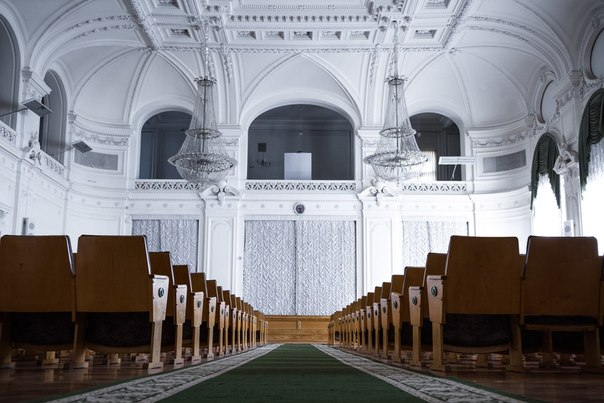
\includegraphics[width=.95\linewidth,valign=t]{my_folder/images//spbpu_whitehall}
	\end{subfigure}
	\hfill %выровнять
	\adjustbox{minipage=1.3em,valign=t}{\subcaption{}\label{fig:spbpu_whitehall-b}}%
	\begin{subfigure}[t]{\dimexpr.3\linewidth-1.3em\relax}
		\centering
		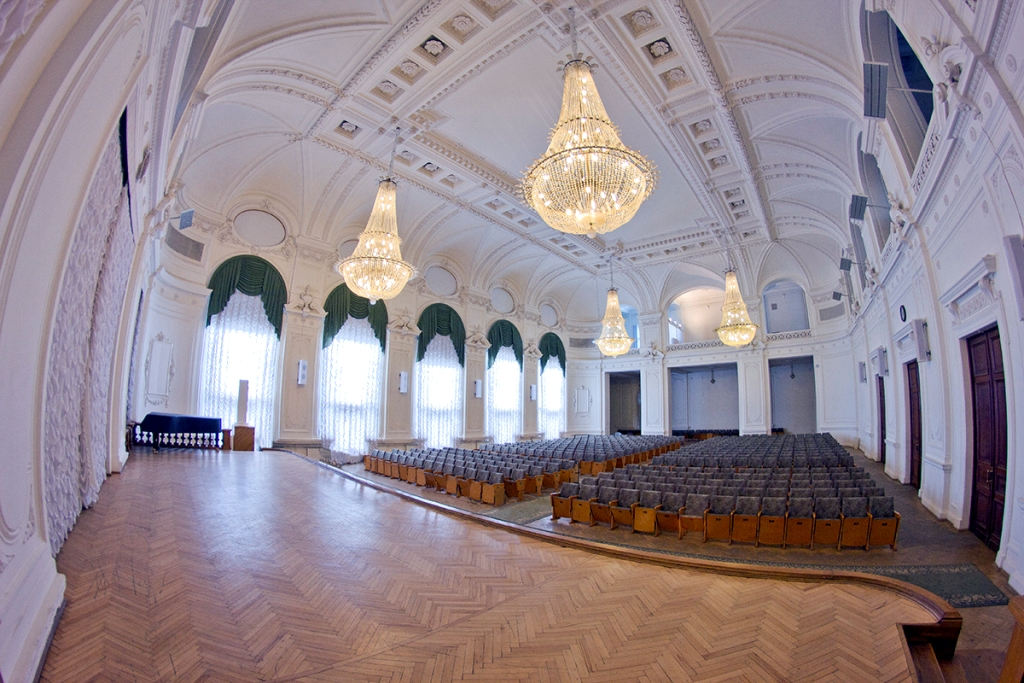
\includegraphics[width=.95\linewidth,valign=t]{my_folder/images//spbpu_whitehall_ligh}
	\end{subfigure}
	\hfill %выровнять
		\adjustbox{minipage=1.3em,valign=t}{\subcaption{}\label{fig:spbpu_whitehall-c}}%
	\begin{subfigure}[t]{\dimexpr.3\linewidth-1.3em\relax}
		\centering
		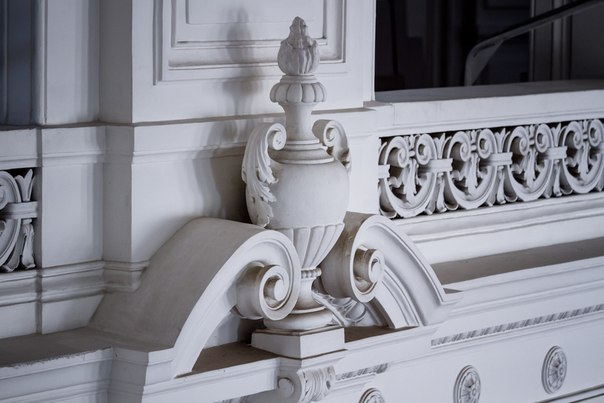
\includegraphics[width=.95\linewidth,valign=t]{my_folder/images//spbpu_whitehall_sculpture}
	\end{subfigure}%
\captionsetup{justification=centering} %центрировать
	\caption{Фотографии Белого зала СПбПУ \cite{spbpu-gallery}, в том числе: {\itshape a} --- со стороны зрителей; {\itshape b} --- со стороны сцены; {\itshape c} --- барельеф}\label{fig:spbpu_whitehall-three-photos}  
\end{figure}

Далее можно ссылаться на три отдельных рисунка: \firef{fig:spbpu_whitehall-a}, \firef{fig:spbpu_whitehall-b} и \firef{fig:spbpu_whitehall-c}. % пример подключения 3х иллюстрации в одном рисунке

Пример ссылок \cite{Article,Book,Booklet,Conference,Inbook,Incollection,Manual,Mastersthesis,Misc,Phdthesis,Proceedings,Techreport,Unpublished,badiou:briefings}, а также ссылок с указанием страниц, на котором отображены номера страниц  \cite[с.~96]{Naidenova2017} или в виде мультицитаты на несколько источников \cites[с.~96]{Naidenova2017}[с.~46]{Ganter1999}. Часть библиографических записей носит иллюстративный характер и не имеет отношения к реальной литературе. 



%\FloatBarrier % заставить рисунки и другие подвижные (float) элементы остановиться

\section{Выводы} \label{ch1:conclusion}

Текст выводов по главе \thechapter.

Кроме названия параграфа <<выводы>> можно использовать (единообразно по всем главам) следующие подходы к именованию последних разделов с результатами по главам:
\begin{itemize}
	\item <<выводы по главе N>>, где N --- номер соответствующей главы;
	\item <<резюме>>;
	\item <<резюме по главе N>>, где N --- номер соответствующей главы.
\end{itemize}

Параграф с изложением выводов по главе \textit{является обязательным}.

%% Вспомогательные команды - Additional commands
%
%\newpage % принудительное начало с новой страницы, использовать только в конце раздела
%\clearpage % осуществляется пакетом <<placeins>> в пределах секций
%\newpage\leavevmode\thispagestyle{empty}\newpage % 100 % начало новой страницы